
%%%%%%%%%%%%%%%%%%%%%%%%%%%%%%%%%%%%%%%%%%%%%%%%%%%%%%%%
%
% Copyright (c) 2003-2008 by University of Queensland
% Earth Systems Science Computational Center (ESSCC)
% http://www.uq.edu.au/esscc
%
% Primary Business: Queensland, Australia
% Licensed under the Open Software License version 3.0
% http://www.opensource.org/licenses/osl-3.0.php
%
%%%%%%%%%%%%%%%%%%%%%%%%%%%%%%%%%%%%%%%%%%%%%%%%%%%%%%%%


\section{3-D Wave Propagation}
\label{WAVE CHAP}

In this next example we want to calculate the displacement field $u\hackscore{i}$ for any time $t>0$ by solving the wave equation:
\index{wave equation}
\begin{eqnarray}\label{WAVE general problem}
\rho u\hackscore{i,tt} - \sigma\hackscore{ij,j}=0
\end{eqnarray}
in a three dimensional block of length $L$ in $x\hackscore{0}$
and $x\hackscore{1}$ direction and height $H$
in $x\hackscore{2}$ direction. $\rho$ is the known density which may be a function of its location.
$\sigma\hackscore{ij}$ is the stress field \index{stress} which in case of an isotropic, linear elastic material is given by
\begin{eqnarray} \label{WAVE stress}
\sigma\hackscore{ij} & = & \lambda u\hackscore{k,k} \delta\hackscore{ij} + \mu ( u\hackscore{i,j} + u\hackscore{j,i})
\end{eqnarray}
where $\lambda$ and $\mu$ are the Lame coefficients 
\index{Lame coefficients} and $\delta\hackscore{ij}$ denotes the Kronecker symbol\index{Kronecker symbol}.
On the boundary the normal stress is given by
\begin{eqnarray} \label{WAVE natural}
\sigma\hackscore{ij}n\hackscore{j}=0
\end{eqnarray}
for all time $t>0$. 

At initial time $t=0$ the displacement 
$u\hackscore{i}$ and the velocity $u\hackscore{i,t}$ are given:
\begin{eqnarray} \label{WAVE initial}
u\hackscore{i}(0,x)= \left\{\begin{array}{cc} U\hackscore{0} & \mbox{for $x$ at point charge, $x\hackscore{C}$} \\ 0 & \mbox{elsewhere}\end{array}  \right. & \mbox{ and } & u\hackscore{i,t}(0,x)=0 \; 
\end{eqnarray}
for all $x$ in the domain. 

Here we are modelling a point source at the point $x\hackscore C$, in the numerical solution we
 set the initial displacement to be $U\hackscore 0$ in a sphere of small radius around the point
 $x\hackscore C$.  

We use an explicit time integration scheme to calculate the displacement field $u$ at 
certain time marks $t^{(n)}$ where $t^{(n)}=t^{(n-1)}+h$ with time step size $h>0$. In the following the upper index ${(n)}$ refers to values at time $t^{(n)}$. We use the Verlet scheme \index{Verlet scheme} with constant time step size $h$
which is defined by
\begin{eqnarray} \label{WAVE dyn 2}
u^{(n)}=2u^{(n-1)}-u^{(n-2)} + h^2 a^{(n)} \\
\end{eqnarray}
for all $n=2,3,\ldots$. It is designed to solve a system of equations of the form
\begin{eqnarray} \label{WAVE dyn 2b} 
u\hackscore{,tt}=G(u)
\end{eqnarray}
where one sets $a^{(n)}=G(u^{(n-1)})$.

In our case $a^{(n)}$ is given by
\begin{eqnarray}\label{WAVE dyn 3}
\rho a^{(n)}\hackscore{i}=\sigma^{(n-1)}\hackscore{ij,j}
\end{eqnarray}
and boundary conditions
\begin{eqnarray} \label{WAVE natural at n}
\sigma^{(n-1)}\hackscore{ij}n\hackscore{j}=0
\end{eqnarray}
derived from \eqn{WAVE natural} where 
\begin{eqnarray} \label{WAVE dyn 3a}
\sigma\hackscore{ij}^{(n-1)} & = & \lambda u^{(n-1)}\hackscore{k,k} \delta\hackscore{ij} + \mu ( u^{(n-1)}\hackscore{i,j} + u^{(n-1)}\hackscore{j,i}).
\end{eqnarray}
Now we have converted our problem for displacement, $u^{(n)}$, into a problem for 
acceleration, $a^(n)$, which now depends 
on the solution at the previous two time steps, $u^{(n-1)}$  and $u^{(n-2)}$.

In each time step we have to solve this problem to get the acceleration $a^{(n)}$, and we will
use the \LinearPDE class of the \linearPDEs to do so. The general form of the PDE defined through
the \LinearPDE class is discussed in \Sec{SEC LinearPDE}. The form which is relevant here is
\begin{equation}\label{WAVE dyn 100}
D\hackscore{ij} a^{(n)}\hackscore{j} = - X\hackscore{ij,j}\; .
\end{equation}
The natural boundary condition
\begin{equation}\label{WAVE dyn 101}
n\hackscore{j}X\hackscore{ij} =0 
\end{equation}
is used. 

With $u=a^{(n)}$ we can identify the values to be assigned to $D$ and $X$:
\begin{equation}\label{WAVE  dyn 6}
\begin{array}{ll}
D\hackscore{ij}=\rho \delta\hackscore{ij}&
X\hackscore{ij}=-\sigma^{(n-1)}\hackscore{ij} \\
\end{array}
\end{equation}


%Remember that \var{y.whereZero()} returns a function which is $1$ for those points $x$ where $y$ is zero
%(up to a certain tolerance, see \Sec{SEC ESCRIPT DATA}) and $0$ for those points where $y$ is not equal to zero.
 
The following script defines a the function \function{wavePropagation} which
implements the Verlet scheme to solve our wave propagation problem. 
The argument \var{domain} which is a \Domain class object
defines the domain of the problem. \var{h} and \var{tend} are the time step size
and the end time of the simulation. \var{lam}, \var{mu} and 
\var{rho} are material properties. 
\begin{python}
from esys.linearPDEs import LinearPDE
from numarray import identity,zeros,ones
from esys.escript import *
from esys.escript.pdetools import Locator
def wavePropagation(domain,h,tend,lam,mu,rho,U0):
   x=domain.getX()
   # ... open new PDE ...
   mypde=LinearPDE(domain)
   mypde.setSolverMethod(LinearPDE.LUMPING)
   kronecker=identity(mypde.getDim())
   #  spherical source at middle of bottom face
   xc=[width/2.,width/2.,0.] 
   # define small radius around point xc
   # Lsup(x) returns the maximum value of the argument x
   src_radius = 0.1*Lsup(domain.getSize())
   print "src_radius = ",src_radius
   dunit=numarray.array([1.,0.,0.]) # defines direction of point source
   mypde.setValue(D=kronecker*rho)
   # ... set initial values ....
   n=0
   # initial value of displacement at point source is constant (U0=0.01)
   # for first two time steps
   u=U0*whereNegative(length(x-xc)-src_radius)*dunit
   u_last=U0*whereNegative(length(x-xc)-src_radius)*dunit
   t=0
   # define the location of the point source
   L=Locator(domain,xc)
   # find potential at point source
   u_pc=L.getValue(u)
   print "u at point charge=",u_pc
   u_pc_x = u_pc[0]
   u_pc_y = u_pc[1]
   u_pc_z = u_pc[2]
   # open file to save displacement at point source
   u_pc_data=open('./data/U_pc.out','w')
   u_pc_data.write("%f %f %f %f\n"%(t,u_pc_x,u_pc_y,u_pc_z))
   while t<tend:
     # ... get current stress ....
     g=grad(u)
     stress=lam*trace(g)*kronecker+mu*(g+transpose(g))
     # ... get new acceleration ....
     mypde.setValue(X=-stress)
     a=mypde.getSolution()
     # ... get new displacement ...
     u_new=2*u-u_last+h**2*a
     # ... shift displacements ....
     u_last=u
     u=u_new
     t+=h
     n+=1
     print n,"-th time step t ",t
     L=Locator(domain,xc)
     u_pc=L.getValue(u)
     print "u at point charge=",u_pc
     u_pc_x=u_pc[0]
     u_pc_y=u_pc[1]
     u_pc_z=u_pc[2]
     # save displacements at point source to file for t > 0
     u_pc_data.write("%f %f %f %f\n"%(t,u_pc_x,u_pc_y,u_pc_z))
     # ... save current acceleration in units of gravity and displacements
     if n==1 or n%10==0: saveVTK("./data/usoln.%i.vtu"%(n/10),acceleration=length(a)/9.81,
     displacement = length(u), Ux = u[0] )
   u_pc_data.close()
\end{python}
Notice that 
all coefficients of the PDE which are independent of time $t$ are set outside the \code{while} 
loop. This is very efficient since it allows the \LinearPDE class to reuse information as much as possible 
when iterating over time.  
 
there are a few new \escript functions in this example: 
\code{grad(u)} returns the gradient $u\hackscore{i,j}$ of $u$ (in fact \var{grad(g)[i,j]}=$=u\hackscore{i,j}$).
There are restrictions on the argument of the \function{grad} function, for instance
the statement \code{grad(grad(u))} will raise an exception.
\code{trace(g)} returns the sum of the main diagonal elements \var{g[k,k]} of \var{g} 
and \code{transpose(g)} returns the matrix transpose of \var{g} (ie. $\var{transpose(g)[i,j]}=\var{g[j,i]}$). 

We initialize the values of \code{u} and \code{u_last} to be $U\hackscore 0$ for a small 
sphere of radius, \code{src_radius} around the point source located at $x\hackscore C$.
These satisfy the initial conditions defined in \eqn{WAVE initial}.

The output \code{U_pc.out} and \code{vtu} files are saved in a directory called \code{data}.
The \code{U_pc.out} stores 4 columns of data: $t,u\hackscore x,u\hackscore y,u\hackscore z$ 
respectively, where $u\hackscore x,u\hackscore y,u\hackscore z$ are the $x\hackscore 0,x\hackscore 1,x\hackscore 2$ components of 
the displacement vector $u$ at the point source. These can be
plotted easily using any plotting package. In gnuplot the command:
\code{plot 'U_pc.out' u 1:2 title 'U_x' w l lw 2, 'U_pc.out' u 1:3 title 'U_y' w l lw 2, 
'U_pc.out' u 1:4 title 'U_z' w l lw 2} will reproduce Figure \ref{WAVE FIG 1}.
%\begin{python}
%u=Vector(0.,ContinuousFunction(domain))
%\end{python}
%declares \var{u} as a vector-valued function of its coordinates 
%in the domain (i.e. with two or three components in the case of 
%a two or three dimensional domain, respectively). The first argument defines the value of the function which is equal
%to $0$ for all vectot components. The second argument \var{ContinuousFunction(domain)} 
%specifies the `smoothness` of the function. In our case we want the displacement field to be 
%a continuous function over the \Domain \var{domain}. On other option would be 
%\var{Function(domain)} in which case continuity is not guaranteed. In fact the 
%argument of the \function{grad} function has to be of the typ \var{ContinuousFunction(domain)} while
%returned function is of the var{Function(domain)} type. For more details see \Sec{SEC ESCRIPT DATA}. 

The statement \code{myPDE.setLumpingOn()}
switches on the use of an aggressive approximation of the PDE operator as a diagonal matrix
formed from the coefficient \var{D}.
The approximation allows, at the cost of 
additional error, very fast 
solution of the PDE. When using \code{setLumpingOn} the presence of \var{A}, \var{B} or \var
{C} will produce wrong results.


One of the big advantages of the Verlet scheme is the fact that the problem to be solved 
in each time step is very simple and does not involve any spatial derivatives (which is what allows us to use lumping in this simulation).
The problem becomes so simple because we use the stress from the last time step rather then the stress which is
actually present at the current time step. Schemes using this approach are called an explicit time integration 
schemes \index{explicit scheme} \index{time integration!explicit}. The 
backward Euler scheme we have used in \Chap{DIFFUSION CHAP} is 
an example of an implicit scheme
\index{implicit scheme} \index{time integration!implicit}. In this case one uses the actual status of 
each variable at a particular time rather then values from previous time steps. This will lead to a problem which is 
more expensive to solve, in particular for non-linear problems. 
Although 
explicit time integration schemes are cheap to finalize a single time step, they need significantly smaller time
steps then implicit schemes and can suffer from stability problems. Therefore they need a 
very careful selection of the time step size $h$.

An easy, heuristic way of choosing an appropriate
time step size is the Courant condition \index{Courant condition} \index{explicit scheme!Courant condition}
which says that within a time step a information should not travel further than a cell used in the 
discretization scheme. In the case of the wave equation the velocity of a (p-) wave is given as
$\sqrt{\frac{\lambda+2\mu}{\rho}}$ so one should choose $h$ from
\begin{eqnarray}\label{WAVE dyn 66}
h= \frac{1}{5} \sqrt{\frac{\rho}{\lambda+2\mu}} \Delta x
\end{eqnarray}
where $\Delta x$ is the cell diameter. The factor $\frac{1}{5}$ is a safety factor considering the heuristics of 
the formula.

The following script uses the \code{wavePropagation} function to solve the
wave equation for a point source located at the bottom face of a block. The width of the block in 
each direction on the bottom face is $10\mbox{km}$ ($x\hackscore 0$ and $x\hackscore 1$ directions ie. \code{l0} and \code{l1}).
The \code{ne} gives the number of elements in $x\hackscore{0}$ and $x\hackscore 1$ directions.  
The depth of the block is aligned with the $x\hackscore{2}$-direction. 
The depth (\code{l2}) of the block in
the $x\hackscore{2}$-direction is chosen so that there are 10 elements and the magnitude of the
of the depth is chosen such that the elements 
become cubic. We chose 10 for the number of elements in $x\hackscore{2}$-direction so that the 
computation would be faster. \code{Brick($n\hackscore 0,  n\hackscore 1, n\hackscore 2,l\hackscore 0,l\hackscore 1,l\hackscore 2$)} is an \finley function which creates a rectangular mesh 
with $n\hackscore 0 \times n\hackscore 1 \times n\hackscore2$ elements over the brick $[0,l\hackscore 0] \times [0,l\hackscore 1] \times [0,l\hackscore 2]$.
\begin{python}
from esys.finley import Brick
ne=32          # number of cells in x_0 and x_1 directions
width=10000.  # length in x_0 and x_1 directions
lam=3.462e9
mu=3.462e9
rho=1154.
tend=60
h=(1./5.)*sqrt(rho/(lam+2*mu))*(width/ne)
print "time step size = ",h
U0=0.01 # amplitude of point source

mydomain=Brick(ne,ne,10,l0=width,l1=width,l2=10.*width/32.)
wavePropagation(mydomain,h,tend,lam,mu,rho,U0)
\end{python}
The script is available as \file{wave.py} in the \ExampleDirectory \index{scripts!\file{wave.py}}. Before running the code make sure you have created a directory called \code{data} in the current
working directory.
To visualize the results from the data directory: 
\begin{verbatim} mayavi -d usoln.1.vtu -m SurfaceMap &\end{verbatim} You can rotate this figure by clicking on it with the mouse and moving it around.
Again use \code{Configure Data} to move backwards and forward in time, and 
also to choose the results (acceleration, displacement or $u\hackscore x$) by using \code{Select Scalar}. Figure \ref{WAVE FIG 2} shows the results for the displacement at various time steps.

\begin{figure}{t!}
\centerline{\includegraphics[width=3.in,angle=270]{figures/WavePC.eps}}
\caption{Amplitude at Point source}
\label{WAVE FIG 1}
\end{figure}

\begin{figure}{t}
\begin{center}
\includegraphics[width=2in,angle=270]{figures/Wavet0.eps}
\includegraphics[width=2in,angle=270]{figures/Wavet1.eps}
\includegraphics[width=2in,angle=270]{figures/Wavet3.eps}
\includegraphics[width=2in,angle=270]{figures/Wavet10.eps}
\includegraphics[width=2in,angle=270]{figures/Wavet30.eps}
\includegraphics[width=2in,angle=270]{figures/Wavet288.eps}
\end{center}
\caption{Selected time steps ($n = 0,1,30,100,300$ and 2880) of a wave propagation over a $10\mbox{km} \times 10\mbox{km} \times 3.125\mbox{km}$ block 
from a point source initially at $(5\mbox{km},5\mbox{km},0)$
with time step size $h=0.02083$. Color represents the displacement.
Here the view is oriented onto the bottom face.
\label{WAVE FIG 2}}
\end{figure}
